\documentclass[12pt,a4paper]{article}

\usepackage{avant,graphicx,color,longtable,fancyvrb,hyperref,amsmath,fancyhdr}
\usepackage[margin=2cm]{geometry}
\usepackage[normalem]{ulem}
\usepackage{pdflscape}
\usepackage{pbox}

\DefineVerbatimEnvironment{Highlighting}{Verbatim}{commandchars=\\\{\}}
\newenvironment{Shaded}{}{}
\newcommand{\KeywordTok}[1]{\textcolor[rgb]{0.00,0.44,0.13}{\textbf{{#1}}}}
\newcommand{\DataTypeTok}[1]{\textcolor[rgb]{0.56,0.13,0.00}{{#1}}}
\newcommand{\DecValTok}[1]{\textcolor[rgb]{0.25,0.63,0.44}{{#1}}}
\newcommand{\BaseNTok}[1]{\textcolor[rgb]{0.25,0.63,0.44}{{#1}}}
\newcommand{\FloatTok}[1]{\textcolor[rgb]{0.25,0.63,0.44}{{#1}}}
\newcommand{\CharTok}[1]{\textcolor[rgb]{0.25,0.44,0.63}{{#1}}}
\newcommand{\StringTok}[1]{\textcolor[rgb]{0.25,0.44,0.63}{{#1}}}
\newcommand{\CommentTok}[1]{\textcolor[rgb]{0.38,0.63,0.69}{\textit{{#1}}}}
\newcommand{\OtherTok}[1]{\textcolor[rgb]{0.00,0.44,0.13}{{#1}}}
\newcommand{\AlertTok}[1]{\textcolor[rgb]{1.00,0.00,0.00}{\textbf{{#1}}}}
\newcommand{\FunctionTok}[1]{\textcolor[rgb]{0.02,0.16,0.49}{{#1}}}
\newcommand{\RegionMarkerTok}[1]{{#1}}
\newcommand{\ErrorTok}[1]{\textcolor[rgb]{1.00,0.00,0.00}{\textbf{{#1}}}}
\newcommand{\NormalTok}[1]{{#1}}

\begin{document}

\title{Scheduler \\ Database Project Report}
\author{Thai Pangsakulyanont \\ Khanet Krongkitichu \\ Lattasit Haritaworn}
\date{November 2013}
\maketitle

\begin{center}
\small This report is part of project work for \textbf{01219331 Database Design \& Programming Course}.
\end{center}

\pagestyle{fancyplain}
\fancyhf{}
\lhead{ \fancyplain{}{Scheduler, Database Project Report} }
\rhead{ \fancyplain{}{\today} }
\rfoot{ \fancyplain{}{\thepage} }

\tableofcontents
\newpage

\newcommand{\NR}{\noalign{\medskip}}
\newcommand{\Code}[1]{\texttt{#1}}
\newcommand{\Tbl}[1]{\subsubsection{Table \texttt{#1}}}

\input{../contents/1-background.md}

\input{../contents/2-vision.md}


\section{Software Tools}

\begin{center}
  \begin{tabular}{ll}

\hline \NR
Tool & Purpose \\\NR
\hline\NR

  draw.io & ER Diagramming \\\NR

  MySQL & Database Management System \\\NR

  PHP & Scripting language on the server \\\NR

  phpMyAdmin & Database development and administration tool \\\NR

  AngularJS & Client-side application framework \\\NR

  DomCrawler & Scraping the registration website's timetable \\\NR

  Facebook PHP SDK & User Authentication and Login with Facebook \\\NR

  pdfLaTeX \\*
  Pygments \\*
  Pandoc & Report authoring tools \\\NR

\hline


  \end{tabular}
\end{center}




\section{ER Diagram}
\begin{center}
  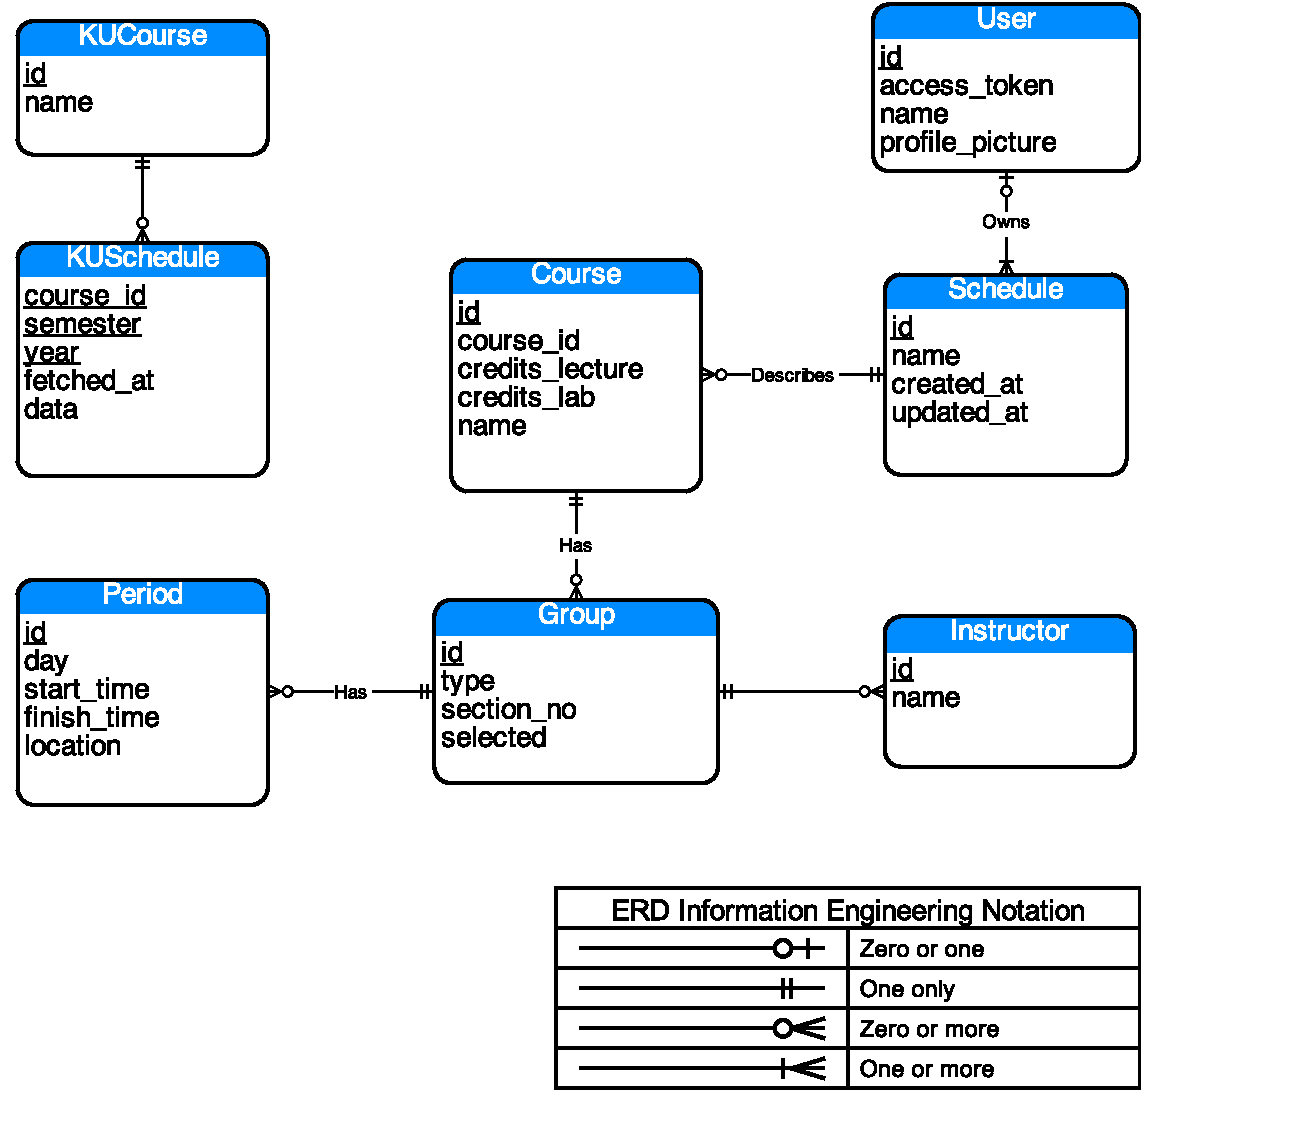
\includegraphics[width=0.8\textwidth]{../../er-diagram.pdf}
\end{center}



\input{../contents/5-1-naming.md}


\subsection{Data Dictionary}

\newcommand{\TblData}[1]{\begin{center}
  \begin{tabular}{llrp{10cm}}
    \hline \NR
    Attribute Name & Data Type & Size & Description \\\NR
    \hline\NR
      #1
    \hline
  \end{tabular}
\end{center}}
\newcommand{\TblCol}[4]{
  \texttt{#1} & \texttt{#2} & #3 & #4 \\\NR
}


% ~ tables

\Tbl{users}

Users sign in by using Facebook.
This table contains the information
of all (identified) users that uses this application.

\TblData{
  \TblCol{\uline{id}}{INT}{11}{
    ID of the user generated by DBMS}
  \TblCol{uid}{VARCHAR}{64}{
    User's Facebook user ID.}
  \TblCol{name}{VARCHAR}{128}{
    User's Facebook name.}
}


\Tbl{schedules}

A user can create many schedules.
This table contains all the schedules in the application.

If the user does not sign in,
then \Code{user\_id} will be \Code{NULL}.


\TblData{
  \TblCol{\uline{id}}{INT}{11}{
    ID of the schedule generated by DBMS.}
  \TblCol{user\_id}{INT}{11}{
    ID of the schedule's owner, or \Code{NULL}
    if the owner chooses not to be identified.}
  \TblCol{name}{TEXT}{-}{
    Name of the schedule.}
  \TblCol{secret}{CHAR}{6}{
    Secret key that must be present in order for anyone to access the schedule.}
  \TblCol{created\_at}{TIMESTAMP}{-}{
    Timestamp representing schedule's creation date and time.}
  \TblCol{updated\_at}{TIMESTAMP}{-}{
    Timestamp representing schedule's last modification date and time.}
}



\Tbl{courses}

A schedule contains many courses.

\TblData{
  \TblCol{\uline{id}}{INT}{11}{
    ID of the course generated by DBMS.}
  \TblCol{schedule\_id}{INT}{11}{
    ID of the schedule that this course belongs to.}
  \TblCol{name}{TEXT}{-}{
    Name of the course.}
  \TblCol{course\_id}{VARCHAR}{20}{
    Course code. For example, in KU, it's something like 01234567.}
  \TblCol{credits\_lecture}{INT}{11}{
    Number of lecture credits for this course.}
  \TblCol{credits\_lab}{INT}{11}{
    Number of lab credits for this course.}
  \TblCol{display\_name}{VARCHAR}{50}{
    Shorter name of the course to display in the timetable view
    (the timetable view has much less space, so we need to have a shorter name
    or an abbreviation).
    It is a blank string (\Code{""}),
    in case the display name isn't needed.}
}



\Tbl{groups}

A course contains many groups (or sections).

\TblData{
  \TblCol{\uline{id}}{INT}{11}{
    ID of the group generated by DBMS.}
  \TblCol{course\_id}{INT}{11}{
    ID of the course that this section belongs to.}
  \TblCol{section\_no}{VARCHAR}{10}{
    The section number of this group.}
  \TblCol{type}{VARCHAR}{20}{
    Type of this section. May be \Code{"Lecture"} or \Code{"Lab"}}
  \TblCol{selected}{TINYINT}{1}{
    \(\begin{cases}
      1 & \text{if the user selected this course,} \\
      0 & \text{otherwise.}
    \end{cases}\)}
}


\Tbl{periods}

In each group, the instructor teaches in many times.

\TblData{
  \TblCol{\uline{id}}{INT}{11}{
    ID of the period generated by DBMS.}
  \TblCol{group\_id}{INT}{11}{
    ID of the group that this period belongs to.}
  \TblCol{day}{INT}{11}{
    The day of the class period. Its value is 0 if Sunday, 1 if Monday, \(\cdots\), and 6 if Sunday.}
  \TblCol{start\_time}{INT}{11}{
    The starting time of this class period.
    Its value is the number of minutes since midnight.
    For example, 9:30 AM is represented as 570.}
  \TblCol{finish\_time}{INT}{11}{
    The finishing time of this class period.
    Its value is the number of minutes since midnight.}
  \TblCol{location}{VARCHAR}{80}{
    Location that this class period is expected to take place.}
}


\Tbl{instructors}

In each group, there are one or many instructors teaching this course
(but usually there's just one).

For simplicity of programming,
same instructor in different courses or different groups
are represented by different rows.

\TblData{
  \TblCol{\uline{id}}{INT}{11}{
    ID of the row generated by DBMS.}
  \TblCol{group\_id}{INT}{11}{
    ID of the group that this row belongs to.}
  \TblCol{name}{VARCHAR}{40}{
    Name of the instructor}
}




\Tbl{ku\_courses}

This table holds all available courses in Kasetsart University's registration system.

\TblData{
  \TblCol{\uline{id}}{CHAR}{8}{
    8-digit course code for this course.}
  \TblCol{name}{INT}{11}{
    The name of the course, as taken from the registration system's website}
}


\Tbl{ku\_timetables}

This table holds the latest schedule data for selected courses in KU.
Each course may contain several timetables. Each timetable can be identified by:

\begin{itemize}
  \item Course ID,
  \item Academic Year, and
  \item Semester Number.
\end{itemize}

Each row in this table contains an encoded timetable,
consisting of all groups, along with its periods and instructors.

This table acts as a cache.
A row is deleted from the database within 1 hour.
The next request must contact KU's system to retrive a newer timetable
and put insert it into the database.

\TblData{
  \TblCol{\uline{ku\_course\_id}}{CHAR}{8}{
    8-digit course code for this timetable.}
  \TblCol{\uline{year}}{INT}{11}{
    The academic year of this timetable.
    Its value is the last two digits of the academic year in B.E.}
  \TblCol{\uline{semester}}{INT}{11}{
    \(\begin{cases}
      0 & \text{if summer semester,} \\
      1 & \text{if first semester,} \\
      2 & \text{if second semester,} \\
      3 & \text{if third semester.}
    \end{cases}\)}
  \TblCol{fetched\_at}{TIMESTAMP}{-}{
    Timestamp representing the date and time that this timetable is retrived.
    The timetable is invalidated within 1 hours after retrieval,
    and is purged from the database.}
  \TblCol{timetable}{TEXT}{-}{
    JSON-encoded timetable data,
    containing all offered groups and its periods,
    number of credits for lecture and lab.}
}











\subsection{Example Data}

\Tbl{ku\_courses}

\begin{center} \input{../contents/ex-ku_courses} \end{center}

\Tbl{users}

\begin{center} \input{../contents/ex-users} \end{center}

\begin{landscape}

  \Tbl{schedules}

  \begin{center} \input{../contents/ex-schedules} \end{center}

  \Tbl{courses}

  \begin{center} \input{../contents/ex-courses} \end{center}

\end{landscape}

\subsubsection{Tables \texttt{groups} and \texttt{instructors}}

\begin{center}
  \input{../contents/ex-groups} \quad \input{../contents/ex-instructors}
\end{center}

\Tbl{periods}

\begin{center} \input{../contents/ex-periods} \end{center}

\newpage

\Tbl{ku\_timetables}

\begin{center} \input{../contents/ex-ku_timetables} \end{center}


\input{../contents/6-example-queries.md}

\end{document}
